% Capítulo 2 - Introducción específica

\chapter{Introducción específica}

\label{Chapter2}

En este capítulo se describen las herramientas de terceros sobre las que se apoyó el trabajo: el lenguaje, los frameworks y las bibliotecas de software, el dataset RadioML 2016.10A junto con el subconjunto que se utilizó, y la infraestructura de cómputo empleada para los entrenamientos y las evaluaciones.

%----------------------------------------------------------------------------------------
%	SECTION 1
%----------------------------------------------------------------------------------------

\section{Frameworks y bibliotecas de IA/ML}
\label{sec:frameworks}

El trabajo se desarrolló en Python, un lenguaje de código abierto administrado por la Python Software Foundation \cite{python2026about}. El código compartido entre los modelos y los barridos de experimentos se implementaron en módulos y scripts de Python, mientras que cada arquitectura quedó documentada en un cuaderno Jupyter, un formato de documento que combina código, resultados y explicaciones en un mismo archivo \cite{kluyver2016jupyter}.

El framework de aprendizaje profundo utilizado fue PyTorch. En esta biblioteca los modelos se definen como programas regulares de Python y las derivadas necesarias para el entrenamiento se calculan mediante diferenciación automática en modo inverso, con soporte para aceleradores de hardware como las GPU (del inglés, \textit{Graphics Processing Unit}) \cite{paszke2019pytorch}. Con PyTorch se definieron, entrenaron y evaluaron todas las arquitecturas comparadas en el trabajo.

La elección de PyTorch se debió a tres motivos. En primer lugar, la biblioteca cuenta con numerosas herramientas para redes neuronales: capas convolucionales y recurrentes (convolución unidimensional, LSTM y GRU), normalización por lotes, regularización por dropout, la entropía cruzada como función de pérdida, optimizadores como Adam, el programador de tasa de aprendizaje ReduceLROnPlateau y cargadores de datos \cite{pytorch2026docs}. Además, las capas se expresan como clases de Python, lo que permite definir capas propias con libertad \cite{paszke2019pytorch}, necesidad que surgió al implementar modelos con bloques no estándar. En segundo lugar, cada uno de estos módulos cuenta con documentación oficial detallada \cite{pytorch2026docs}. Por último, fue el framework empleado en gran parte de la especialización, por lo que su manejo previo permitió reducir el tiempo de desarrollo.

También se utilizo biblioteca scikit-learn que reúne algoritmos de aprendizaje automático supervisado y no supervisado, e incluye iteradores que generan los índices de entrenamiento y prueba de una partición de los datos, entre ellos la validación cruzada estratificada \cite{pedregosa2011scikit}. En el trabajo se utilizó para dividir el dataset en conjuntos de entrenamiento, validación y prueba, para codificar las etiquetas de las clases y para calcular las matrices de confusión. También se utilizó para los modelos clásicos, basados en máquinas de vectores de soporte (SVM, del inglés \textit{Support Vector Machine}) con los clasificadores SVC y LinearSVC \cite{sklearn2026docs}. Las características de entrada de estos modelos se estandarizaron con StandardScaler, que lleva cada característica a media cero y varianza unitaria \cite{sklearn2026docs}; los pasos de procesamiento se encadenaron con Pipeline \cite{pedregosa2011scikit,sklearn2026docs} y los hiperparámetros se seleccionaron con GridSearchCV, que evalúa todas las combinaciones de una grilla de valores \cite{pedregosa2011scikit,sklearn2026docs}.

% TODO: citar Harris 2020 (NumPy), Virtanen 2020 (SciPy) y Hunter 2007 (Matplotlib) una vez verificados (ver referencias_cap2.md)
Para el manejo de arreglos numéricos se utilizó NumPy y para el procesamiento de señales se utilizó SciPy. La visualización de los resultados se realizó con Matplotlib y con seaborn, una biblioteca de visualización estadística de datos \cite{waskom2021seaborn}.

La metadata del dataset, almacenada en formato parquet, se leyó con polars, una biblioteca de tablas de datos (\textit{DataFrame}) cuyo núcleo está escrito en Rust \cite{polars2026docs}.

Por último, se empleó la biblioteca rfml, desarrollada por Flowers y Headley \cite{flowers2019rfml}. Se trata de una biblioteca de aprendizaje automático para radiofrecuencia sobre PyTorch, distribuida con licencia BSD-3, que incluye conversores para cargar los datasets abiertos de DeepSig \cite{flowers2019rfml}. En el trabajo se utilizó para cargar los datos y para obtener el modelo de línea base. El resto del código fue desarrollado por el autor y se describe en el capítulo \ref{Chapter3}.

%----------------------------------------------------------------------------------------
%	SECTION 2
%----------------------------------------------------------------------------------------

\section{Datasets y datos de entrenamiento}
\label{sec:datasets}

El dataset utilizado fue RadioML 2016.10A, publicado por DeepSig. Se trata de un conjunto de datos sintético, generado con GNU Radio, que contiene 11 modulaciones, 8 digitales y 3 analógicas, a distintos niveles de SNR \cite{deepsig2016datasets}. Es una versión más limpia y normalizada de RadioML 2016.04C, al que reemplaza \cite{deepsig2016datasets}. El procedimiento de generación del dataset original se describe en O'Shea et al. \cite{oshea2016convolutional}, y se resume a continuación.

Según se describe en dicho trabajo, se modularon conjuntos de datos reales de voz y texto y, en el caso de las modulaciones digitales, los datos se aleatorizaron por bloques para que los bits fueran equiprobables. Cada señal atravesó un modelo de canal que incluye desvanecimiento multicamino variable en el tiempo, deriva aleatoria de los osciladores de frecuencia portadora y de reloj de muestreo, y ruido gaussiano blanco aditivo, implementado con los bloques de canal de GNU Radio. Finalmente, la señal se segmentó en ventanas rectangulares cortas \cite{oshea2016convolutional}. Los efectos del canal producen desplazamientos temporales, cambios de escala, rotaciones y giros de la señal recibida \cite{oshea2016convolutional}.

Las modulaciones digitales del dataset son 8PSK, BPSK, CPFSK, GFSK, PAM4, QAM16, QAM64 y QPSK. El dataset contiene 1.000 ejemplos por cada combinación de modulación y nivel de SNR, con 20 niveles entre -20 y 18 dB en pasos de 2 dB, lo que totaliza 220.000 ejemplos. Cada ejemplo está formado por 128 muestras complejas, almacenadas como dos canales, I y Q. En el trabajo se utilizó únicamente el subconjunto de las 8 modulaciones digitales, con 160.000 ejemplos. En la tabla \ref{tab:dataset} se resumen las características del dataset y del subconjunto utilizado. Las cantidades de ejemplos y la forma de cada uno se obtuvieron de los archivos del dataset empleados en el trabajo.

\begin{table}[h]
	\centering
	\caption{Características de RadioML 2016.10A y del subconjunto utilizado.}
	\begin{tabular}{l l}
		\toprule
		\textbf{Característica} & \textbf{Valor} \\
		\midrule
		Editor & DeepSig Inc. \\
		Generación & Sintética, con GNU Radio \\
		Licencia & CC BY-NC-SA 4.0 \\
		Modulaciones del dataset & 11 (8 digitales y 3 analógicas) \\
		Modulaciones utilizadas & 8 digitales \\
		Niveles de SNR & 20, de -20 a 18 dB en pasos de 2 dB \\
		Ejemplos por modulación y nivel de SNR & 1.000 \\
		Ejemplos del dataset completo & 220.000 \\
		Ejemplos del subconjunto utilizado & 160.000 \\
		Ejemplos por modulación (subconjunto) & 20.000 \\
		Ejemplos por nivel de SNR (subconjunto) & 8.000 \\
		Forma de cada ejemplo & 2 canales (I y Q) de 128 muestras \\
		\bottomrule
	\end{tabular}
	\label{tab:dataset}
\end{table}

La distribución del subconjunto es uniforme, con la misma cantidad de ejemplos para cada modulación y cada nivel de SNR. En la figura \ref{fig:iq_mod}\footnote{Elaboración propia a partir de los ejemplos del dataset RadioML 2016.10A de DeepSig.} se presenta un ejemplo de cada modulación digital a 18 dB de SNR en el plano IQ, con las amplitudes normalizadas por el valor máximo de cada ejemplo. Los puntos no forman constelaciones nítidas porque el canal introduce rotaciones, giros y desplazamientos de la señal \cite{oshea2016convolutional}.

\begin{figure}[htbp]
	\centering
	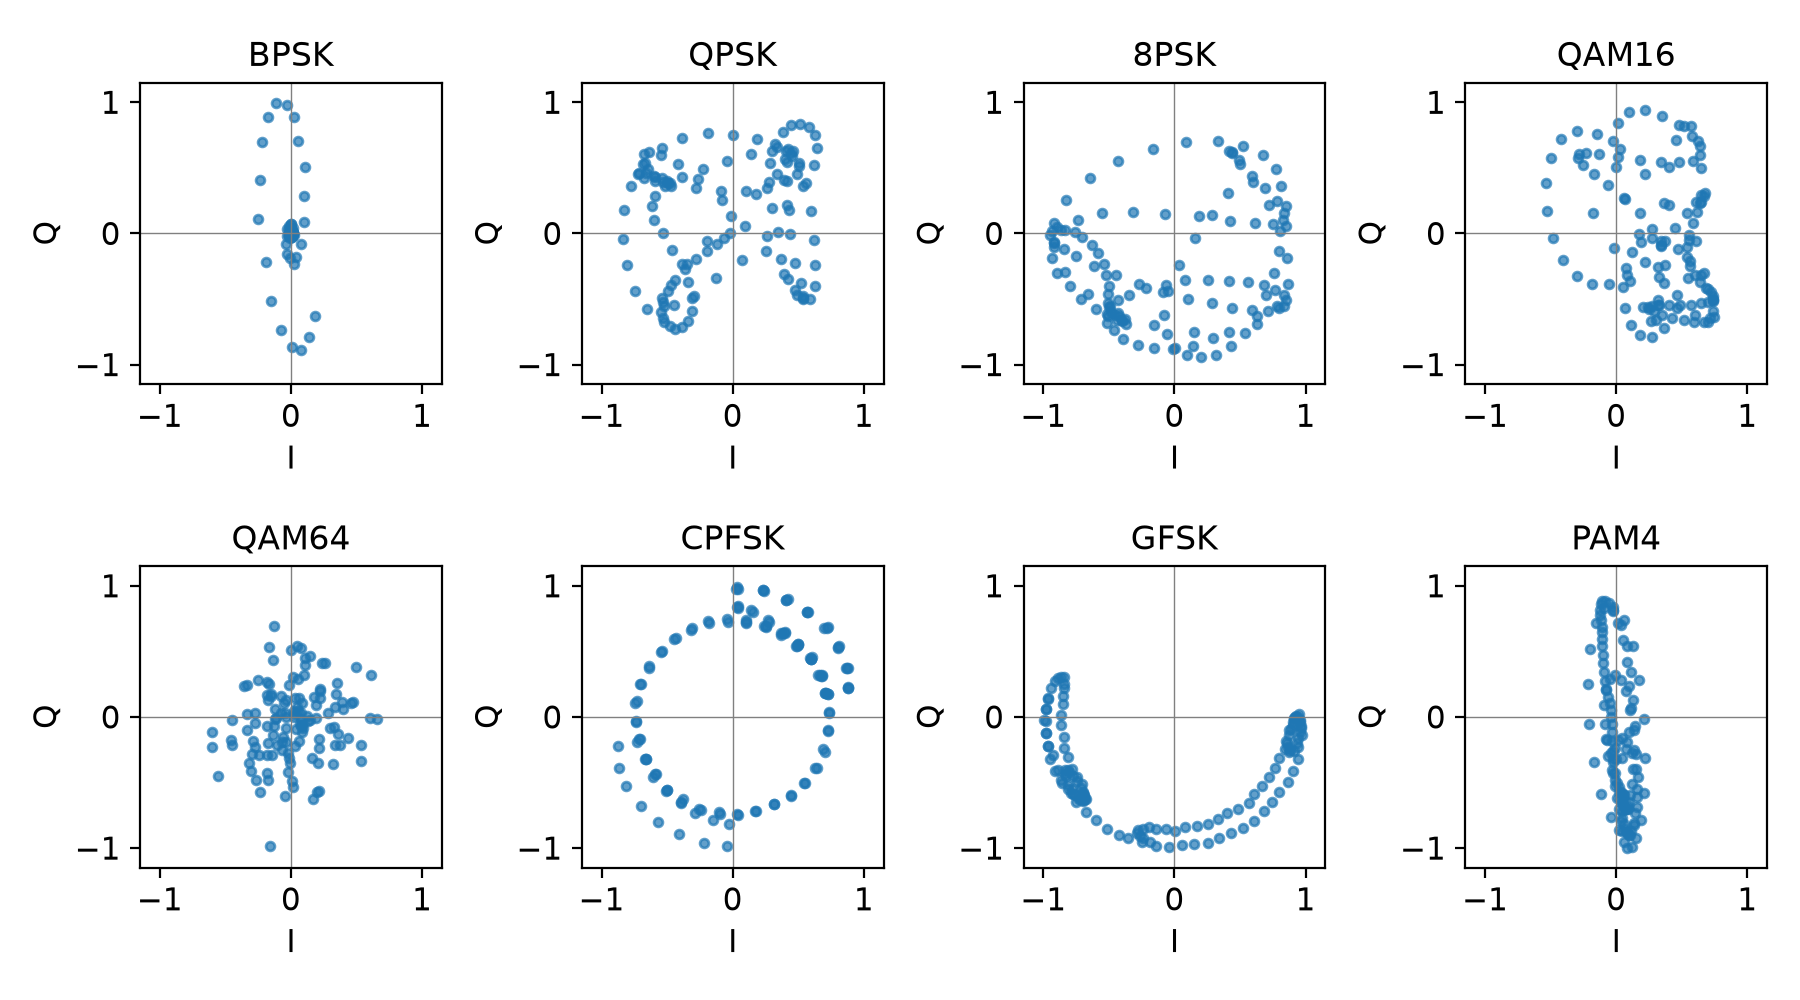
\includegraphics[width=\textwidth]{./Figures/iq_por_modulacion.png}
	\caption{Ejemplo de cada modulación digital del dataset a 18 dB de SNR en el plano IQ.}
	\label{fig:iq_mod}
\end{figure}

En la figura \ref{fig:iq_snr}\footnote{Elaboración propia a partir de los ejemplos del dataset RadioML 2016.10A de DeepSig.} se muestra la misma modulación, QPSK, a distintos niveles de SNR. A 0 dB ya no se distingue la estructura observada a 18 dB, y a -10 y -20 dB los puntos forman una nube sin estructura visible.

\begin{figure}[htbp]
	\centering
	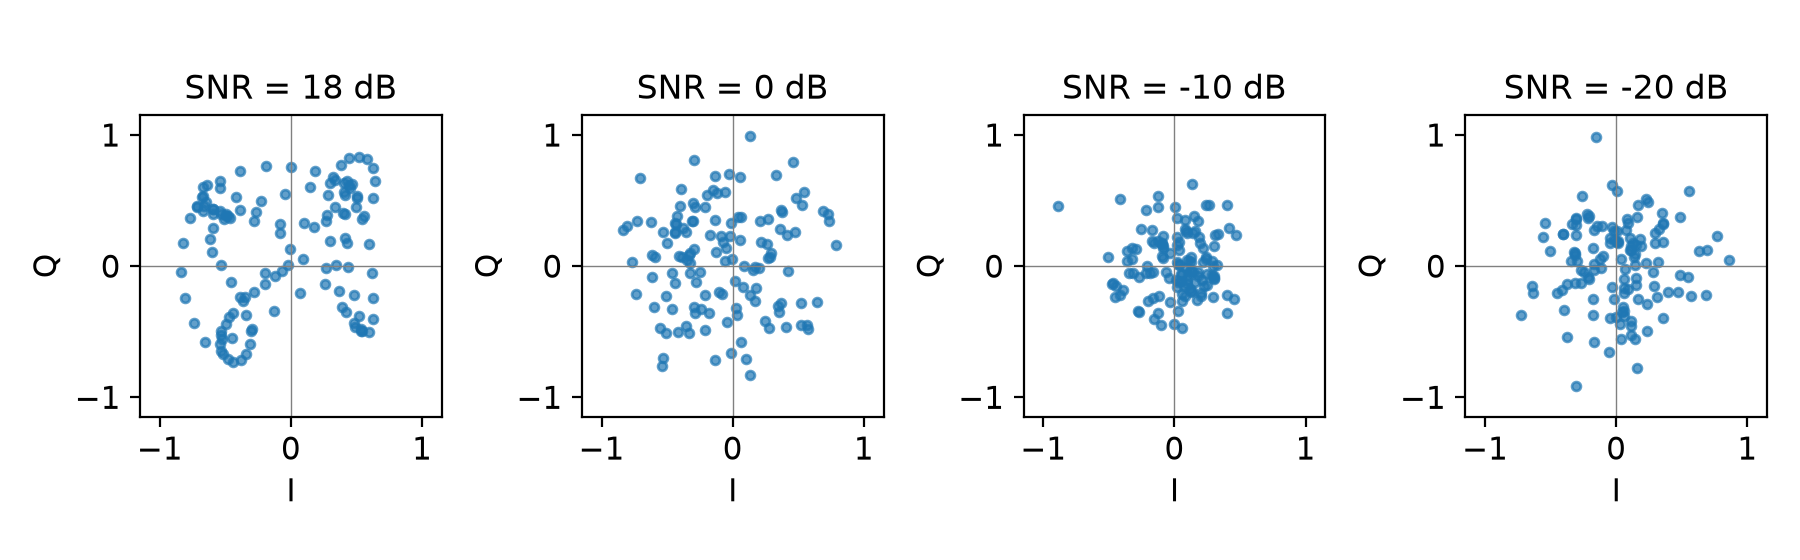
\includegraphics[width=\textwidth]{./Figures/iq_qpsk_snr.png}
	\caption{Ejemplo de la modulación QPSK a distintos niveles de SNR en el plano IQ.}
	\label{fig:iq_snr}
\end{figure}

El dataset se distribuye bajo la licencia Creative Commons Atribución, No Comercial, Compartir Igual 4.0 (CC BY-NC-SA 4.0) \cite{deepsig2016datasets}. Esta licencia restringe su uso a fines no comerciales, condición que el presente trabajo cumple por su carácter académico.

DeepSig advierte que este dataset, producto de una investigación académica de 2016, tiene errores conocidos y no se utiliza en sus productos \cite{deepsig2016datasets}. Además, los autores del dataset original señalan que el entrenamiento con datos reales es importante y valioso, y lo plantean como trabajo futuro \cite{oshea2016convolutional}. Por este motivo, el desempeño sobre señales reales capturadas con un receptor queda fuera del alcance del trabajo.

Además del dataset de terceros, en parte de los experimentos se utilizaron señales sintéticas generadas con un programa desarrollado por el autor, con el fin de dar mayor robustez al entrenamiento. Este programa se describe en el capítulo \ref{Chapter3}.

%----------------------------------------------------------------------------------------
%	SECTION 3
%----------------------------------------------------------------------------------------

\section{Infraestructura de cómputo}
\label{sec:infraestructura}

Los entrenamientos y las evaluaciones se ejecutaron en una computadora personal con sistema operativo Windows 11, procesador AMD Ryzen 5 7600 de 6 núcleos y 12 hilos, 15,7 GB de memoria RAM y una GPU AMD Radeon RX 6700. Estos valores se obtuvieron del propio sistema operativo.

Para aprovechar la GPU se utilizó DirectML a través del paquete torch-directml, que permite entrenar e inferir con PyTorch en GPU compatibles con DirectX 12 \cite{microsoft2026directml}. Microsoft indica que esta solución se encuentra en vista previa pública \cite{microsoft2026directml}, y AMD documenta su instalación para tarjetas Radeon RX en Windows mediante un entorno virtual de Python \cite{amd2025pytorchdirectml}. La última versión publicada del paquete es la 0.2.5.dev240914, de septiembre de 2024, y sus instaladores abarcan hasta Python 3.12 \cite{microsoft2024torchdirectml}. Por este motivo se creó un entorno virtual aparte, con Python 3.12, para las ejecuciones en GPU, mientras que el entorno principal utiliza una versión más reciente de Python y ejecuta en CPU. En la tabla \ref{tab:entornos} se resumen ambos entornos.

\begin{table}[h]
	\centering
	\caption{Entornos de ejecución utilizados.}
	\begin{tabular}{l c c l}
		\toprule
		\textbf{Entorno} & \textbf{Python} & \textbf{PyTorch} & \textbf{Dispositivo} \\
		\midrule
		Principal & 3.13.14 & 2.12.1 (CPU) & CPU \\
		DirectML & 3.12.10 & 2.4.1 (CPU) y torch-directml & GPU AMD Radeon RX 6700 \\
		\bottomrule
	\end{tabular}
	\label{tab:entornos}
\end{table}

Las capas LSTM y GRU de PyTorch produjeron errores de ejecución sobre DirectML, por lo que los modelos recurrentes se entrenaron siempre en CPU. El resto de las arquitecturas se pudo ejecutar en ambos dispositivos.
